\chapter{Statistics}
\section{Collecting data}
\section{Measures of central tendency}
\subsection{Mean}
\subsection{Median}
\subsection{Mode}
\begin{exercises}{}{
    \begin{enumerate}[noitemsep, label=\textbf{\arabic*}.]
    \item Calculate the mean, median and mode of the following data sets:
      \begin{enumerate}[noitemsep, label=\textbf{(\alph*)} ]
      \item $2;~5;~8;~8;~11;~13;~22;~23;~27$
      \item $15;~17;~24;~24;~26;~28;~31;~43$
      \item $4;~11;~3;~15;~11;~13;~25;~17;~2;~11$
      \item $24;~35;~28;~41;~32;~49;~31$
      \end{enumerate}
    \item The ages of $15$ runners of the Comrades Marathon were recorded:
      \begin{equation*}
        31;~42;~28;~38;~45;~51;~33;~29;~42;~26;~34;~56;~33;~46;~41
      \end{equation*}
      Calculate the mean, median and modal age.
    \item In the first of a series of jars, there is $1$ sweet. In the
      second jar, there are $3$ sweets. The mean number of sweets in the
      first two jars is $2$.
      \begin{enumerate}[noitemsep, label=\textbf{(\alph*)} ]
      \item If the mean number of sweets in the first three jars is $3$, how
        many sweets are there in the third jar?
      \item If the mean number of sweets in the first four jars is $4$, how
        many sweets are there in the fourth jar?
      \end{enumerate}
    \item Find a set of five ages for which the mean age is $5$, the modal
      age is $2$ and the median age is $3$ years.
    \item Four friends each have some marbles. They work out that the mean
      number of marbles they have is $10$. One friend leaves with $4$
      marbles. How many marbles do the remaining friends have together?
    \end{enumerate}
\practiceinfo
\par 
\par \begin{tabular}[h]{cccccc}
(1.) lgv  &  (2.) liZ  &  (3.) liB  &  (4.) lac  &  (5.) lax \end{tabular}
}
\end{exercises}


 \begin{solutions}{}{
\begin{enumerate}[itemsep=5pt, label=\textbf{\arabic*}. ] 


\item solution 1
\item solution 2
\item solution 3
\item solution 4
\item solution 5

\end{enumerate}}
\end{solutions}


\section{Grouping data}
\begin{exercises}{}{
    \begin{enumerate}[itemsep=5pt, label=\textbf{\arabic*}. ]
    \item  A class experiment was conducted and $50$ learners were asked to
      guess the number of sweets in a jar. The following guesses were
      recorded
      \\
      \begin{center}
        \begin{tabular}{|c|c|c|c|c|c|c|c|c|c|} \hline
          56 & 49 & 40 & 11 & 33 & 33 & 37 & 29 & 30 & 59 \\ \hline
          21 & 16 & 38 & 44 & 38 & 52 & 22 & 24 & 30 & 34 \\\hline
          42 & 15 & 48 & 33 & 51 & 44 & 33 & 17 & 19 & 44 \\\hline
          47 & 23 & 27 & 47 & 13 & 25 & 53 & 57 & 28 & 23 \\\hline
          36 & 35 & 40 & 23 & 45 & 39 & 32 & 58 & 22 & 40 \\\hline
        \end{tabular}
      \end{center}
      \begin{enumerate}[noitemsep, label=\textbf{(\alph*)} ]
      \item
        Draw up a grouped frequency table using the intervals
        $10 < x \le 20$;\ $20 < x \le 30$;\ $30 < x \le 40$;\ 
        $40 < x \le 50$;and \ $50 < x \le 60$.
      \item Draw the histogram corresponding to the frequency table of the
        grouped data.
      \end{enumerate}
    \end{enumerate}
\practiceinfo
\par 
\par \begin{tabular}[h]{cccccc}
(1.) lgv & \end{tabular}
}
\end{exercises}


 \begin{solutions}{}{
\begin{enumerate}[itemsep=5pt, label=\textbf{\arabic*}. ] 


\item solution 1

\end{enumerate}}
\end{solutions}


\begin{exercises}{}{
  \begin{enumerate}[itemsep=8pt, label=\textbf{\arabic*}.]
  \item Consider the following grouped data and calculate the mean,
    the modal group and the median group.
\\
    \begin{center}
      \begin{tabular}{|c|c|}\hline
        \textbf{Mass (kg)} & \textbf{Count} \\\hline
        $40 < m \le 45$ & $7$ \\\hline
        $45 < m \le 50$ & $10$ \\\hline
        $50 < m \le 55$ & $15$ \\\hline
        $55 < m \le 60$ & $12$ \\\hline
        $60 < m \le 65$ & $6$ \\\hline
      \end{tabular}
    \end{center}
  \item Find the mean, the modal group and the median group in this
    data set of how much time people needed to complete a game.
\\
    \begin{center}
      \begin{tabular}{|c|c|} \hline
       \textbf{Time (s)} & \textbf{Count} \\ \hline
        $35 < t \le 45$ & $5$ \\\hline
        $45 < t \le 55$ & $11$ \\\hline
        $55 < t \le 65$ & $15$ \\\hline
        $65 < t \le 75$ & $26$ \\\hline
        $75 < t \le 85$ & $19$ \\\hline
        $85 < t \le 95$ & $13$ \\\hline
        $95 < t \le 105$ & $6$ \\\hline
      \end{tabular}
    \end{center}
\item The histogram below shows the number of passengers that travel in Alfred's minibus taxi per week.\\
Calculate
\begin{enumerate}[noitemsep, label=\textbf{(\alph*)} ]
\item the modal interval
\item the total number of passengers to travel in Alfred's taxi
\item an estimate of the mean
\item an estimate of the median
\item if it is estimated that every passenger travelled an average distance of $5$ km, how much money would Alfred have made if he charged R~$3,50$ per km?
\end{enumerate}
\begin{center}
\scalebox{1} % Change this value to rescale the drawing.
{
\begin{pspicture}(0,-5.1475)(9.378126,5.1075)
\definecolor{color5165b}{rgb}{0.7725490196078432,0.7725490196078432,0.7725490196078432}
\rput(1.3781264,-3.8925){\psaxes[linewidth=0.028222222,arrowsize=0.05291667cm 2.0,arrowlength=1.4,arrowinset=0.4,tickstyle=bottom,ticksize=0.10583333cm,dx=1.0cm,dy=1.0cm,Dx=100,Dy=2,Ox=300]{<->}(0,0)(-1,-1)(8,9)}
\psframe[linewidth=0.02,dimen=outer,fillstyle=solid,fillcolor=color5165b](3.392293,-1.8890625)(2.372293,-3.8890624)
\psframe[linewidth=0.02,dimen=outer,fillstyle=solid,fillcolor=color5165b](4.412293,-0.8890625)(3.372293,-3.8890624)
\psframe[linewidth=0.02,dimen=outer,fillstyle=solid,fillcolor=color5165b](5.412293,2.1309376)(4.372293,-3.8890624)
\psframe[linewidth=0.02,dimen=outer,fillstyle=solid,fillcolor=color5165b](6.392293,4.1309376)(5.372293,-3.8890624)
\psframe[linewidth=0.02,dimen=outer,fillstyle=solid,fillcolor=color5165b](7.392293,0.1309375)(6.372293,-3.8890624)
\psframe[linewidth=0.02,dimen=outer,fillstyle=solid,fillcolor=color5165b](8.392293,-2.8690624)(7.372293,-3.8890624)
\rput(5.369637,-4.9225){No. of passengers}
\rput{89.854546}(0.73185694,0.38878262){\rput(0.13573053,0.5775){Count}}
\end{pspicture} 
}
\end{center}
  \end{enumerate}
\practiceinfo
\par 
\par \begin{tabular}[h]{cccccc}
(1.) lgv  &  (2.) liZ  &  (3.) liB  \end{tabular}
}
\end{exercises}


 \begin{solutions}{}{
\begin{enumerate}[itemsep=5pt, label=\textbf{\arabic*}. ] 


\item solution 1
\item solution 2
\item solution 3

\end{enumerate}}
\end{solutions}


\section{Dispersion}
\subsection{Range}
\subsection{Percentiles}
\subsection{Percentiles for grouped data}
\subsection{Ranges}
\begin{exercises}{}{
  \begin{enumerate}[noitemsep, label=\textbf{\arabic*}.]
  \item Find the range of the data set
    \begin{equation*}
      \{1;\ 2;\ 3;\ 4;\ 4;\ 4;\ 5;\ 6;\ 7;\ 8;\ 8;\ 9;\ 10;\ 10\}
    \end{equation*}
  \item What are the quartiles of this data set?
    \begin{equation*}
      \{3;\ 5;\ 1;\ 8;\ 9;\ 12;\ 25;\ 28;\ 24;\ 30;\ 41;\ 50\}
    \end{equation*}
  \item A class of $12$ students writes a test and the results are as
    follows:
    \begin{equation*}
      20;\ 39;\ 40;\ 43;\ 43;\ 46;\ 53;\ 58;\ 63;\ 70;\ 75;\ 91
    \end{equation*}
    Find the range, quartiles and the interquartile range.
  \item Three sets of data are given:
    \begin{itemize}  
    \item \textbf{Data set 1:} $\{9;\ 12;\ 12;\ 14;\ 16;\ 22;\ 24\}$
    \item \textbf{Data set 2:} $\{7;\ 7;\ 8;\ 11;\ 13;\ 15;\ 16;\ 16\}$
    \item \textbf{Data set 3:} $\{11;\ 15;\ 16;\ 17;\ 19;\ 19;\ 22;\ 24;\ 27\}$
    \end{itemize}
    For each data set find:
    \begin{enumerate}[noitemsep, label=\textbf{(\alph*)} ]
    \item the range
    \item the lower quartile
    \item the interquartile range
    \item the semi-interquartile range
    \item the median
    \item the upper quartile
    \end{enumerate}
  \end{enumerate}
\practiceinfo
\par 
\par \begin{tabular}[h]{cccccc}
(1.) lgv  &  (2.) liZ  &  (3.) liB  &  (4.) lac  & \end{tabular}
}
\end{exercises}


 \begin{solutions}{}{
\begin{enumerate}[itemsep=5pt, label=\textbf{\arabic*}. ] 


\item solution 1
\item solution 2
\item solution 3
\item solution 4
\item solution 5
\item solution 6
\item solution 7

\end{enumerate}}
\end{solutions}


\section{Combining different measures}
\begin{exercises}{}{
    \begin{enumerate} [itemsep=6pt, label=\textbf{\arabic*}.]
    \item Lisa is working in a computer store. She sells the following
      number of computers each month:
      \begin{equation*}
        \{27;\ 39;\ 3;\ 15;\ 43;\ 27;\ 19;\ 54;\ 65;\ 23;\ 45;\ 16\}
      \end{equation*}
      Give the five number summary and box-and-whisker plot of Lisa's
      sales.
    \item Zithulele works as a telesales person. He keeps a record of the
      number of sales he makes each month. The data below show how much he
      sells each month.
      \begin{equation*}
        \{49;\ 12;\ 22;\ 35;\ 2;\ 45;\ 60;\ 48;\ 19;\ 1;\ 43;\ 12\}
      \end{equation*}
      Give the five number summary and box-and-whisker plot of Zithulele's
      sales.
    \item Hannah has worked as a florist for nine months. She sold the
      following number of wedding bouquets:
      \begin{equation*}
        \{16;\ 14;\ 8;\ 12;\ 6;\ 5;\ 3;\ 5;\ 7\}
      \end{equation*}
      Give the five number summary of Hannah's sales.
    \item Use the diagram below to determine the five number summary:
      \begin{enumerate}[noitemsep, label=\textbf{(\alph*)} ]
      \item 
    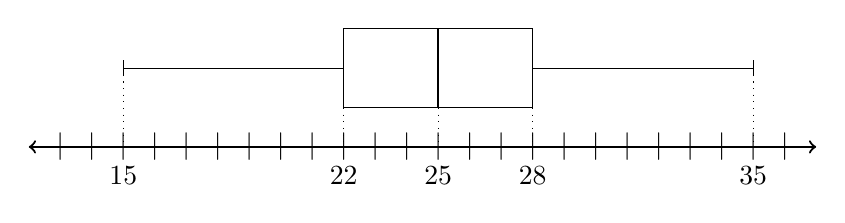
\begin{tikzpicture}[xscale=0.4]
      \def\median{25}
      \def\firstquartile{22}
      \def\thirdquartile{28}
      \def\minimum{15}
      \def\maximum{35}
      \draw (\firstquartile, -0.5 ) rectangle ( \thirdquartile,0.5);
      \draw[thick] ( \median,-0.5) -- ( \median,0.5);
      \draw (    \firstquartile, 0) -- (\minimum,0   );
      \draw ( \minimum, -0.1) -- (       \minimum, 0.1);
      \draw (  \thirdquartile, 0) -- (   \maximum, 0);
      \draw ( \maximum, -0.1) -- (      \maximum, 0.1 );
      \draw[thick,<->] (12,-1) -- (37,-1);
      \foreach \x in {\minimum, \firstquartile, \median, \thirdquartile, \maximum} {
        \draw (\x,-1.6) -- (\x, -1.6) node[anchor=south] {$\x$};
      }
      \foreach \x in {13,14,...,36} {
        \draw (\x,-1.3) -- (\x, -1.3) node[anchor=south] {$|$};
      }
      \draw[dotted] ( \maximum, 0) -- ( \maximum, -1);
      \draw[dotted] ( \thirdquartile, 0) -- ( \thirdquartile, -1);
      \draw[dotted] (\median, 0)  -- ( \median, -1);
      \draw[dotted] (\firstquartile, 0) -- ( \firstquartile, -1);
      \draw[dotted] ( \minimum, 0) -- ( \minimum, -1);
    \end{tikzpicture}
\item 
    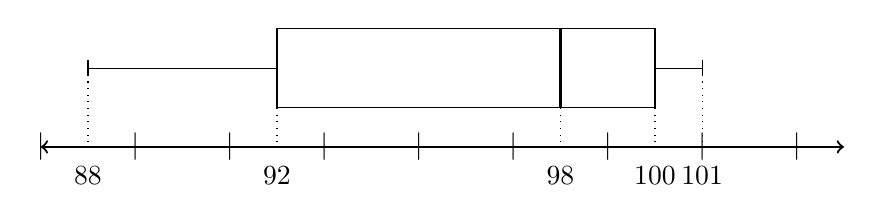
\begin{tikzpicture}[xscale=0.6]
      \def\median{98}
      \def\firstquartile{92}
      \def\thirdquartile{100}
      \def\minimum{88}
      \def\maximum{101}
      \draw (\firstquartile, -0.5 ) rectangle ( \thirdquartile,0.5);
      \draw[thick] ( \median,-0.5) -- ( \median,0.5);
      \draw (    \firstquartile, 0) -- (\minimum,0   );
      \draw ( \minimum, -0.1) -- (       \minimum, 0.1);
      \draw (  \thirdquartile, 0) -- (   \maximum, 0);
      \draw ( \maximum, -0.1) -- (      \maximum, 0.1 );
      \draw[thick,<->] (87,-1) -- (104,-1);
      \foreach \x in {\minimum, \firstquartile, \median, \thirdquartile, \maximum} {
        \draw (\x,-1.6) -- (\x, -1.6) node[anchor=south] {$\x$};
      }
      \foreach \x in {87,89,...,104} {
        \draw (\x,-1.3) -- (\x, -1.3) node[anchor=south] {$|$};
      }
      \draw[dotted] ( \maximum, 0) -- ( \maximum, -1);
      \draw[dotted] ( \thirdquartile, 0) -- ( \thirdquartile, -1);
      \draw[dotted] (\median, 0)  -- ( \median, -1);
      \draw[dotted] (\firstquartile, 0) -- ( \firstquartile, -1);
      \draw[dotted] ( \minimum, 0) -- ( \minimum, -1);
    \end{tikzpicture}
\end{enumerate}
\end{enumerate}
\practiceinfo
\par 
\par \begin{tabular}[h]{cccccc}
(1.) lgv  &  (2.) liZ  &  (3.) liB  &  (4.) lac \end{tabular}
}
\end{exercises}


 \begin{solutions}{}{
\begin{enumerate}[itemsep=5pt, label=\textbf{\arabic*}. ] 


\item solution 1
\item solution 2
\item solution 3
\item solution 4

\end{enumerate}}
\end{solutions}


\begin{eocexercises}{}
  \begin{enumerate}[itemsep=6pt, label=\textbf{\arabic*}.]
  \item 
  In a park, the tallest $7$ trees in a park have heights in metres of
    $41$; $60$; $47$; $42$; $44$; $42$; and $47$. Find the median of
    their heights.
  \item The students in Ndeme's class have the following ages: $5$;
    $6$; $7$; $5$; $4$; $6$; $6$; $6$; $7$; $4$. Find the mode of
    their ages.
  \item An engineering company has designed two different types of
    engines for motorbikes. The two different motorbikes are tested
    for the time (in seconds) it takes for them to accelerate from $0$
    km/h to $60$ km/h.
    \begin{center}
      \begin{tabular}{|@{\hspace{0.1cm}}c@{\hspace{0.1cm}}|@{\hspace{0.1cm}}c@{\hspace{0.1cm}}|@{\hspace{0.1cm}}c@{\hspace{0.1cm}}|@{\hspace{0.1cm}}c@{\hspace{0.1cm}}|@{\hspace{0.1cm}}c@{\hspace{0.1cm}}|@{\hspace{0.1cm}}c@{\hspace{0.1cm}}|@{\hspace{0.1cm}}c@{\hspace{0.1cm}}|@{\hspace{0.1cm}}c@{\hspace{0.1cm}}|@{\hspace{0.1cm}}c@{\hspace{0.1cm}}|@{\hspace{0.1cm}}c@{\hspace{0.1cm}}|@{\hspace{0.1cm}}c@{\hspace{0.1cm}}|} \hline
        & \textbf{Test 1} & \textbf{Test 2} & \textbf{Test 3} & \textbf{Test 4} & \textbf{Test 5} & \textbf{Test 6} & \textbf{Test 7} &\textbf{Test 8} & \textbf{Test 9} & \textbf{Test 10} \\\hline
        \textbf{Bike 1} & $1,55$ & $1,00$ & $0,92$ & $0,80$ & $1,49$ & $0,71$ & $1,06$ & $0,68$ & $0,87$ & $1,09$ \\\hline
        \textbf{Bike 2} & $0,9$ & $1,0$ & $1,1$ & $1,0$ & $1,0$ & $0,9$ & $0,9$ & $1,0$ & $0,9$ & $1,1$ \\\hline
      \end{tabular}
    \end{center}
\vspace {8pt}\\
\begin{enumerate}[noitemsep, label=\textbf{(\alph*)} ]
    \item Which measure of central tendency should be used for this
      information?
    \item Calculate the measure of central tendency that you chose in
      the previous question, for each motorbike.
    \item Which motorbike would you choose based on this information?
      Take note of the accuracy of the numbers from each set of tests.
    \end{enumerate}
  \item In a traffic survey, a random sample of $50$ motorists were
    asked the distance they drove to work daily. This information is
    shown in the table below.\\
    \begin{center}
      \begin{tabular}{|c|c|} \hline
        \textbf{Distance (km)} & \textbf{Count} \\ \hline
        $0 < d \le 5$ & $4$ \\ \hline
        $5 < d \le 10$ & $5$ \\\hline
        $10 < d \le 15$ & $9$ \\\hline
        $15 < d \le 20$ & $10$ \\\hline
        $20 < d \le 25$ & $7$ \\\hline
        $25 < d \le 30$ & $8$ \\\hline
        $30 < d \le 35$ & $3$ \\\hline
        $35 < d \le 40$ & $2$ \\\hline
        $40 < d \le 45$ & $2$ \\\hline
      \end{tabular}
    \end{center}
\vspace {8pt}\\
     \begin{enumerate}[noitemsep, label=\textbf{(\alph*)} ]
    \item Find the approximate mean of the data.
    \item What percentage of samples had a speed of
      \begin{enumerate}[noitemsep, label=\textbf{\roman*}. ]
      \item less than $16$ km?
      \item more than $30$ km?
      \item between $16$ km and $30$ km daily?
      \end{enumerate}
\item Draw a histogram to represent the data
    \end{enumerate}
  \item A company wanted to evaluate the training programme in its
    factory. They gave the same task to trained and untrained
    employees and timed each one in seconds.
\\
    \begin{center}
      \begin{tabular}{|l|c|c|c|c|c|} \hline
        \textbf{Trained} & 121 & 137 & 131 & 135 & 130 \\ \hline
                         & 128 & 130 & 126 & 132 & 127 \\\hline
                         & 129 & 120 & 118 & 125 & 134 \\\hline
        \textbf{Untrained} & 135 & 142 & 126 & 148 & 145 \\\hline
                           & 156 & 152 & 153 & 149 & 145 \\\hline
                           & 144 & 134 & 139 & 140 & 142 \\\hline
      \end{tabular}
    \end{center}
\vspace {8pt}\\
    \begin{enumerate}[noitemsep, label=\textbf{(\alph*)} ]
    \item Find the medians and quartiles for both sets of data.
    \item Find the interquartile range for both sets of data.
    \item Comment on the results.
    \item Draw a box-and-whisker diagram for each data set to illustrate the five number summary.
    \end{enumerate}
  \item A small firm employs nine people. The annual salaries of the employers are:
\\
    \begin{center}
      \begin{tabular}{|r|r|r|} \hline
        R $600~ 000$ & R $250~ 000$ & R $200~ 000$ \\\hline
        R $120 ~000 $& R $100~ 000$ & R $100 ~000$ \\\hline
        R $100 ~000$ & R  $90~ 000$ & R  $80 ~000$ \\\hline
      \end{tabular}
    \end{center}
\vspace {8pt}\\
    \begin{enumerate}[noitemsep, label=\textbf{(\alph*)} ]
    \item Find the mean of these salaries.
    \item Find the mode.
    \item Find the median.
    \item Of these three figures, which would you use for
      negotiating salary increases if you were a trade union
      official? Why?
    \end{enumerate}
  \end{enumerate}
\practiceinfo
\par 
\par \begin{tabular}[h]{cccccc}
(1.) lgv  &  (2.) liZ  &  (3.) liB  &  (4.) lac  &  (5.) lax  &  (6.) laa \end{tabular}
\end{eocexercises}


 \begin{solutions}{}{
\begin{enumerate}[itemsep=5pt, label=\textbf{\arabic*}. ] 


\item solution 1
\item solution 2
\item solution 3
\item solution 4
\item solution 5
\item solution 6
\item solution 7
\item solution 8
\item solution 9

\end{enumerate}}
\end{solutions}


